\vspace{-2em}
Abrigado no coração de uma cidade glamourosa, um lugar onde os viajantes mais exigentes do mundo vêm para descansar e recarregar as energias, ergue-se um hotel que é ao mesmo tempo um destino e uma cápsula do tempo: o Grande Hotel Infinita. Era um edifício antigo e magnífico, infinitamente alto e largo, onde a história e o luxo se encontravam. Um lugar onde cada hóspede podia escapar das exigências do mundo moderno e reabastecer suas energias em um ambiente de elegância atemporal. Por causa de seu tamanho e idade, o hotel não tinha elevadores de passageiros, apenas uma quantidade infinita de escadas conectando todos os andares. Para proporcionar maior conveniência, o hotel havia instalado recentemente um pequeno e barulhento elevador de carga conectado a cada quarto. Os hóspedes podiam ligar para a recepção para pedir lanches, bebidas ou toalhas limpas, e seu pedido seria entregue através do elevador de carga.

O saguão, com tetos altíssimos, apresentava uma grande escadaria de mármore que parecia subir para sempre. Um enorme lustre lançava uma luz quente e dourada, criando uma atmosfera encantadora. A recepção era uma obra-prima de mogno esculpido, gerida por funcionários em uniformes impecáveis. Na recepção, sentava-se Henrietta, uma hipopótamo de bom coração. Seu assistente, Bernard, um rato mensageiro diligente, esperava ao lado com carrinhos de bagagem polidos, aguardando o próximo hóspede. Eles eram os dois únicos funcionários do hotel. Com um número infinito de quartos para manterem em ordem, eles tinham que lidar com um fluxo interminável de hóspedes chegando e partindo a toda hora. Era um dever que cumpriam com maestria, graças à sua organização impecável e ao compromisso com a harmonia.

\clearpage
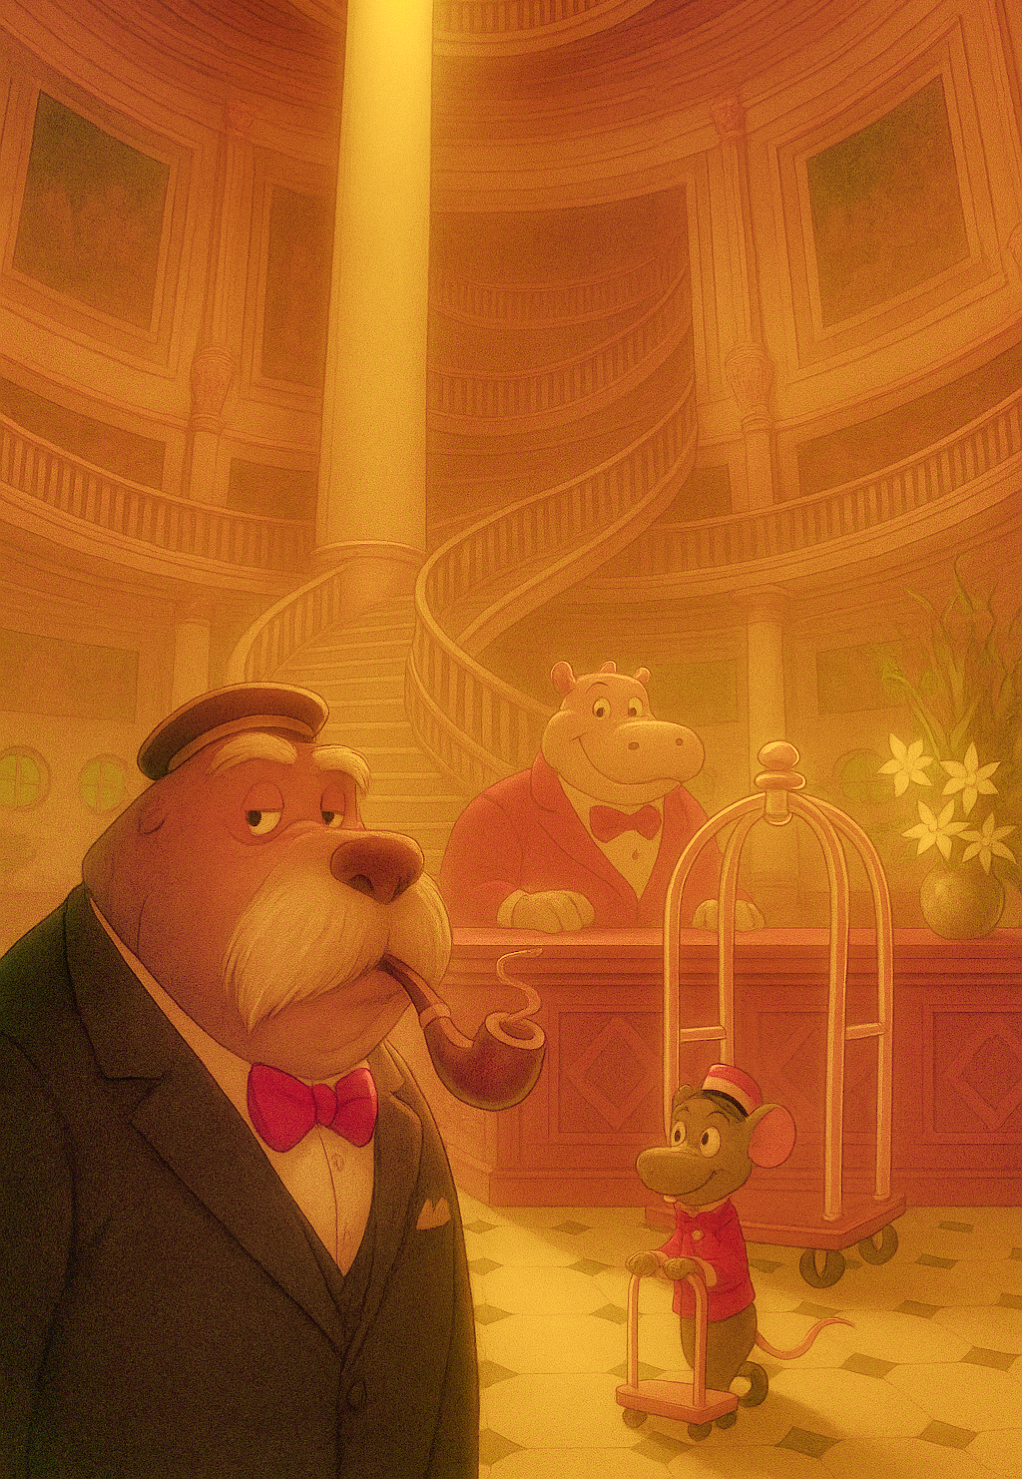
\includepdf[pages={1},
            pagecommand={\thispagestyle{fancy}}, % Apply your custom 'fancy' style
            fitpaper=true,
            noautoscale
           ]{walrus.pdf}

Na noite anterior ao feriado, um distinto leão-marinho fumando um cachimbo foi o último hóspede a chegar. Ele parecia terrivelmente cansado ao entrar. Henrietta, sempre acolhendo os novos hóspedes com afeto, o cumprimentou com um sorriso largo.

``É um prazer recebê-lo no Grande Hotel Infinita'', ela disse. ``Um lugar onde a busca incessante se desfaz, para que você descanse e encontre paz.''
%``Um lugar onde a busca incessante fica para trás, onde você pode descansar e deixar o redemoinho dos turbulentos sonhos para trás.''

``Oh, é tudo que eu preciso'', o leão-marinho respondeu com um suspiro de alívio.

``Nosso hotel está bem cheio hoje, mas o senhor está com sorte, Sr. Leão-Marinho! O primeiro quarto no primeiro andar acaba de ficar vago!'' Henrietta exclamou. ``Nosso ágil Bernard irá ajudá-lo a chegar ao seu quarto imediatamente.''

Bernard o levou ao seu quarto, onde ele desfrutou de uma noite maravilhosamente tranquila.

\vspace{4em}
Na manhã seguinte, era o início de um feriado nacional prolongado, o primeiro após um longo inverno. A equipe do hotel começou o dia com um tipo especial de entusiasmo. Todos estavam ansiosos, aguardando a primeira onda de hóspedes. Este hotel antigo e glamouroso estava acordado e pronto para dar as boas-vindas a um novo dia e criar novas memórias. Mas o que deveria ter sido um momento de descanso e tranquilidade se transformou em uma grande confusão, com muitos hóspedes reclamando de seus tesouros desaparecidos.
